\indent Para corroborar la performance de nuestro algoritmo del inciso A, trabajamos con distintos tipos de grafos.\\

Como la complejidad calculada fue O(E * E * V) decidimos fijar V y tener E movil.\\
Trabajando con grafos circulares variando el tamaño de entrada entre 0 y 10000 y corriendo la misma medición varias veces sacamos un promedio del mismo para obtener datos  más relevantes y obtuvimos el siguiente resultado:

\vspace*{0.3cm} \vspace*{0.3cm}
  \begin{center}
 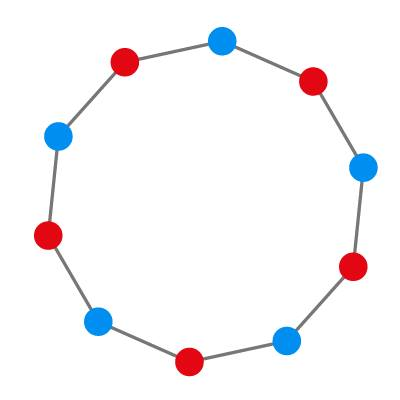
\includegraphics[scale=0.5]{./ej4/circular.jpg}
 	{\\Gráfico 4.4.1 - Grafo circular}
  \end{center}
  \vspace*{0.3cm}
  
  \vspace*{0.3cm} \vspace*{0.3cm}
  \begin{center}
 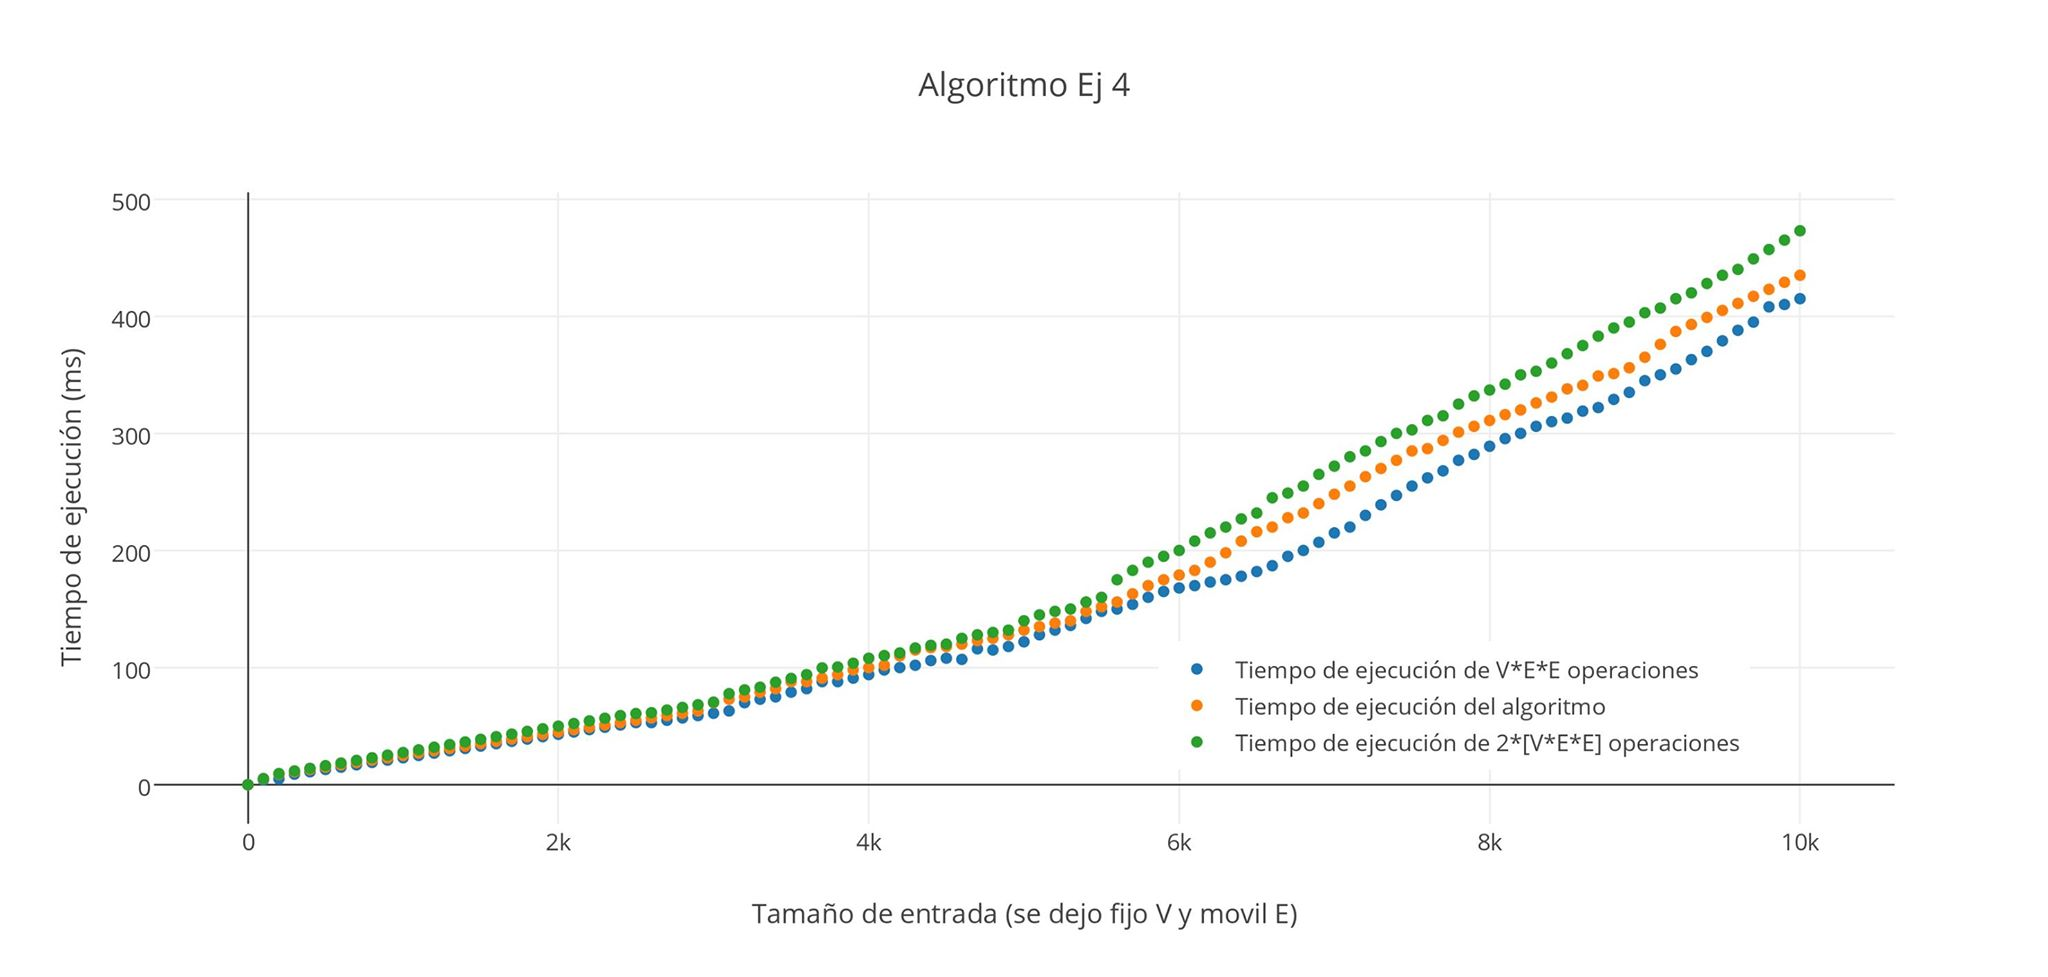
\includegraphics[scale=0.28]{./ej4/circular2.jpg}
 	{Gráfico 4.4.2 - Medición grafo circular}
  \end{center}
  \vspace*{0.3cm}


En la figura 4.4.1 se puede observar el tipo de grafo que utilizamos. En la figura 4.4.2, se puede ver como el tiempo de ejecución de nuestro algoritmo se encuentra entre los tiempos de realizar (E * E * V)  operaciones y 2 (E * E * V)  demostrando como en este tipo de grafo la complejidad calculada de nuestro algoritmo fue correcta.\\




Trabajando con grafos completos variando el tamaño de entrada entre 0 y 10000 y realizando la misma medición varias veces sacamos un promedio del mismo para obtener datos más consistentes y obtuvimos el siguiente resultado:

\vspace*{0.3cm} \vspace*{0.3cm}
  \begin{center}
 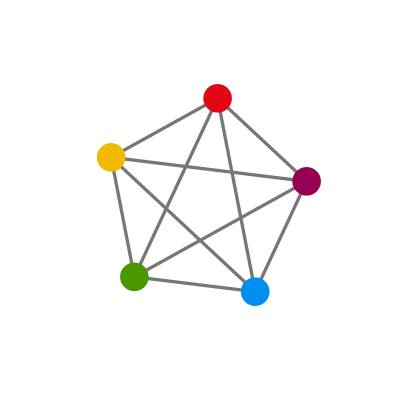
\includegraphics[scale=0.5]{./ej4/completo.jpg}
 	{\\Gráfico 4.4.3 - Grafo completo}
  \end{center}
  \vspace*{0.3cm}
  
  \vspace*{0.3cm} \vspace*{0.3cm}
  \begin{center}
 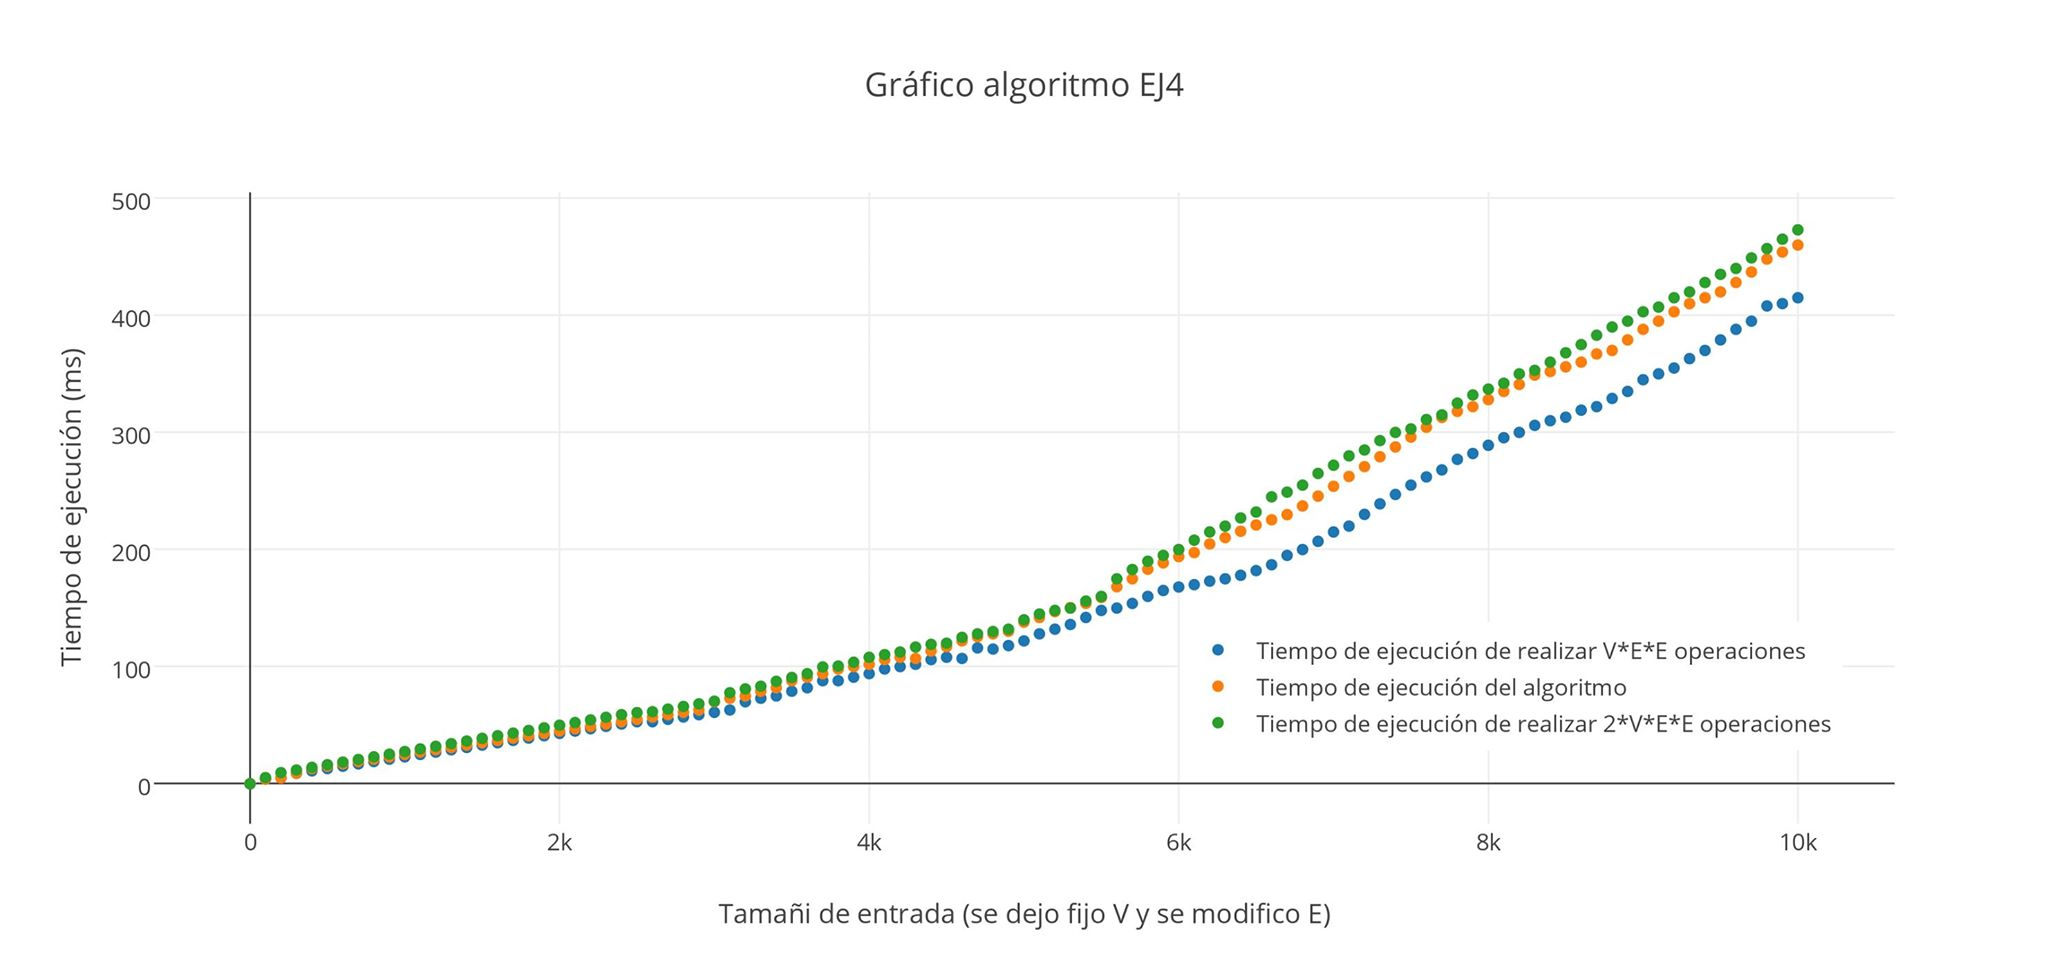
\includegraphics[scale=0.28]{./ej4/completo2.jpg}
 	{Gráfico 4.4.4 - Medición con grafo completo}
  \end{center}
  \vspace*{0.3cm}

En la figura 4.4.3 se puede observar el tipo de grafo que utilizamos. En la figura 4.4.4, se puede ver como el tiempo de ejecución de nuestro algoritmo es un poco mayor que un grafo circular, ya que tenemos más nodos interconectados y a pesar de esta situación nos mantenemos dentro de los tiempos estipulados corroborando la complejidad calculada.\\


Para el algoritmo del inciso B decidimos utilizar los mismos tipos de gráficos para realizar las respectivas mediciones y luego realizamos un gráfico comparativo de los mismos para chequear que tan "buenas" resultaban las soluciones.\\

Se detalla a continuación lo enunciado:\\

En este algoritmo la complejidad teórica resultante fue O(E * E * V * C), y por lo tanto decidimos fijar V y C y tener E movil.\\

Trabajando con grafos circulares variando el tamaño de entrada entre 0 y 10000 y corriendo la misma medición varias veces sacamos un promedio del mismo para obtener datos  más consisos y obtuvimos el siguiente resultado:

\vspace*{0.3cm} \vspace*{0.3cm}
  \begin{center}
 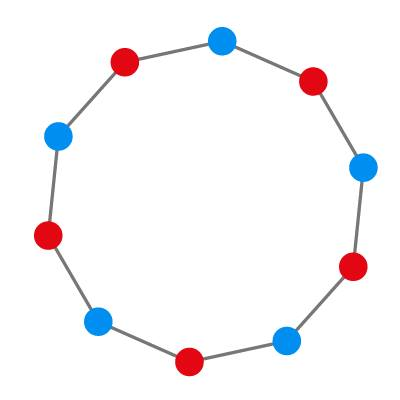
\includegraphics[scale=0.5]{./ej4/circular.jpg}
 	{\\Gráfico 4.4.4 - Grafo circular}
  \end{center}
  \vspace*{0.3cm}
  
  \vspace*{0.3cm} \vspace*{0.3cm}
  \begin{center}
 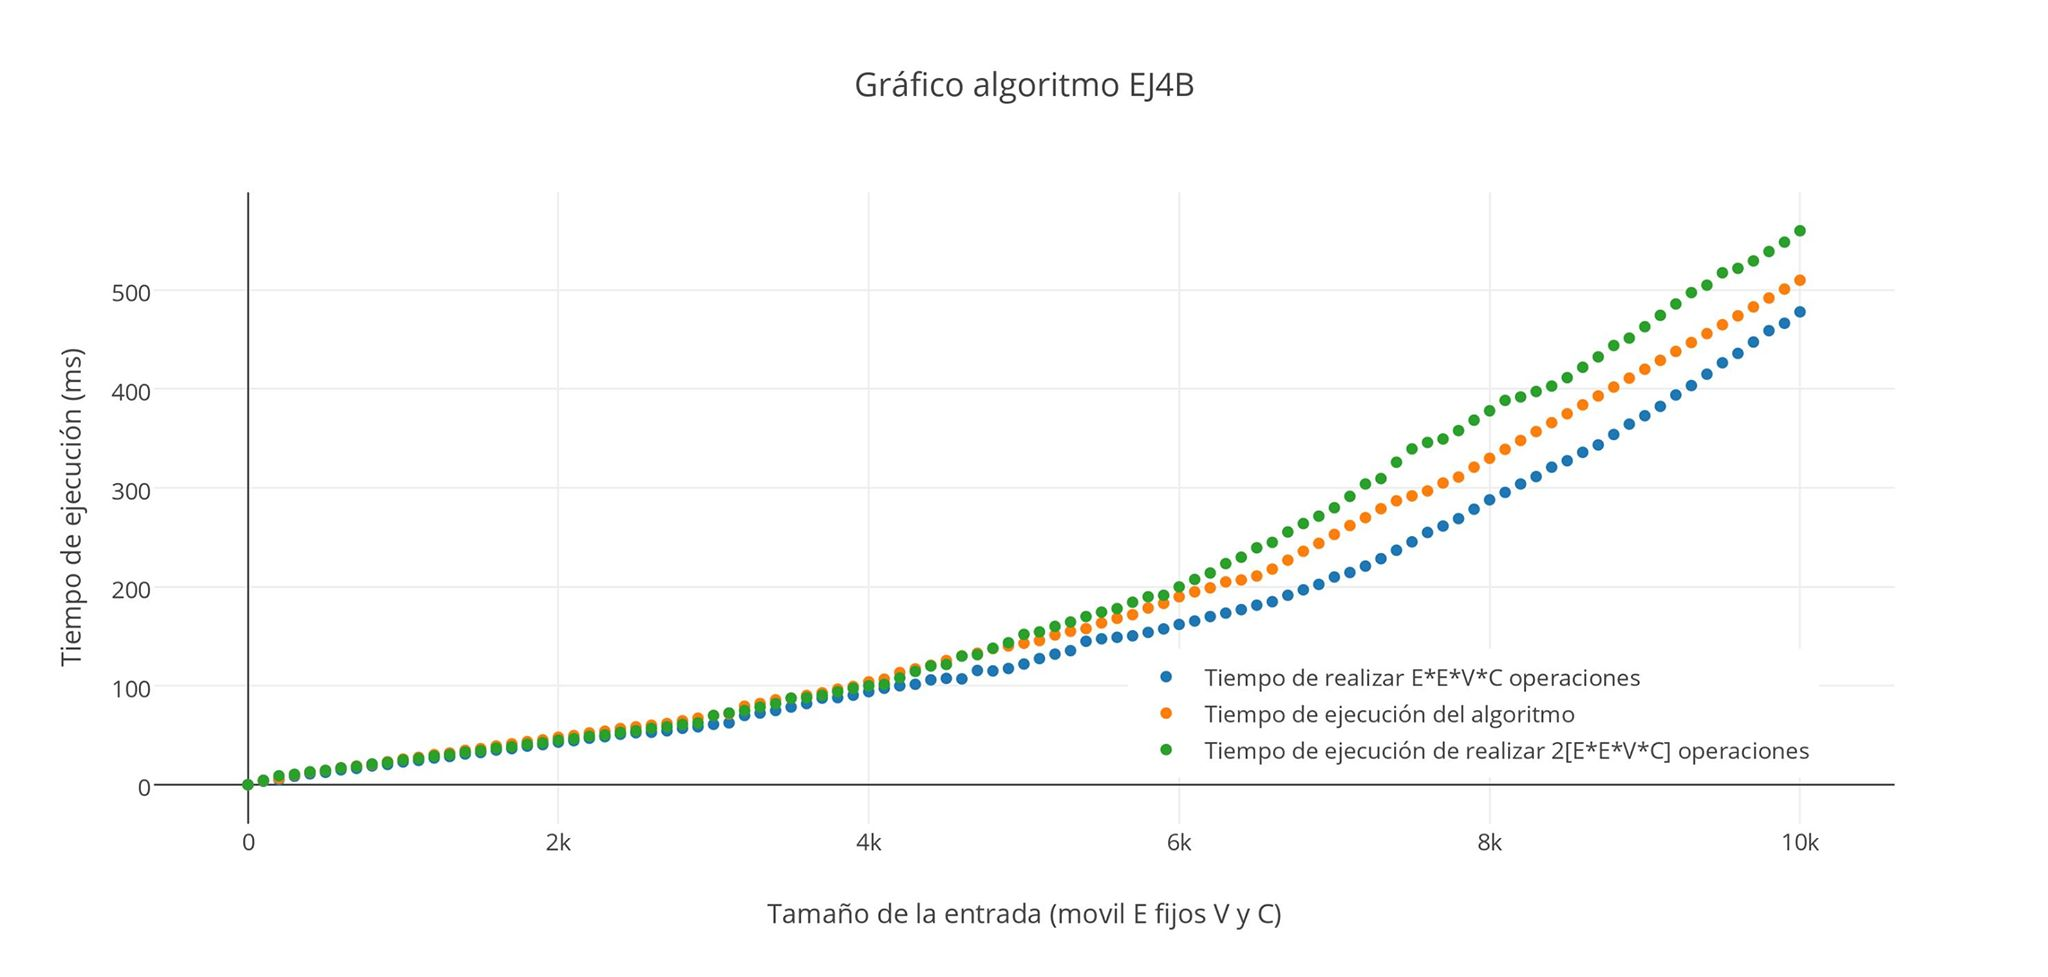
\includegraphics[scale=0.28]{./ej4/circular2b.jpg}
 	{Gráfico 4.4.5 - Medición grafo circular}
  \end{center}
  \vspace*{0.3cm}


En la figura 4.4.4 se puede observar el tipo de grafo que utilizamos. En la figura 4.4.5, se puede ver como el tiempo de ejecución de nuestro algoritmo se encuentra acotado por los tiempos de realizar (E * E * V * C)  operaciones y 2 (E * E * V * C)  demostrando como en este tipo de grafo la complejidad calculada de nuestro algoritmo fue correcta.\\


Trabajando con grafos completos variando el tamaño de entrada entre 0 y 10000 y realizando la misma medición varias veces sacamos un promedio del mismo para obtener datos más consistentes y obtuvimos el siguiente resultado:

\vspace*{0.3cm} \vspace*{0.3cm}
  \begin{center}
 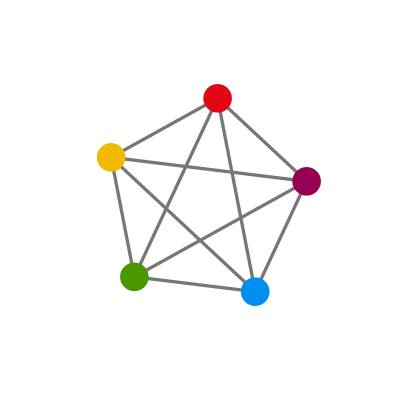
\includegraphics[scale=0.5]{./ej4/completo.jpg}
 	{\\Gráfico 4.4.6 - Grafo completo}
  \end{center}
  \vspace*{0.3cm}
  
  \vspace*{0.3cm} \vspace*{0.3cm}
  \begin{center}
 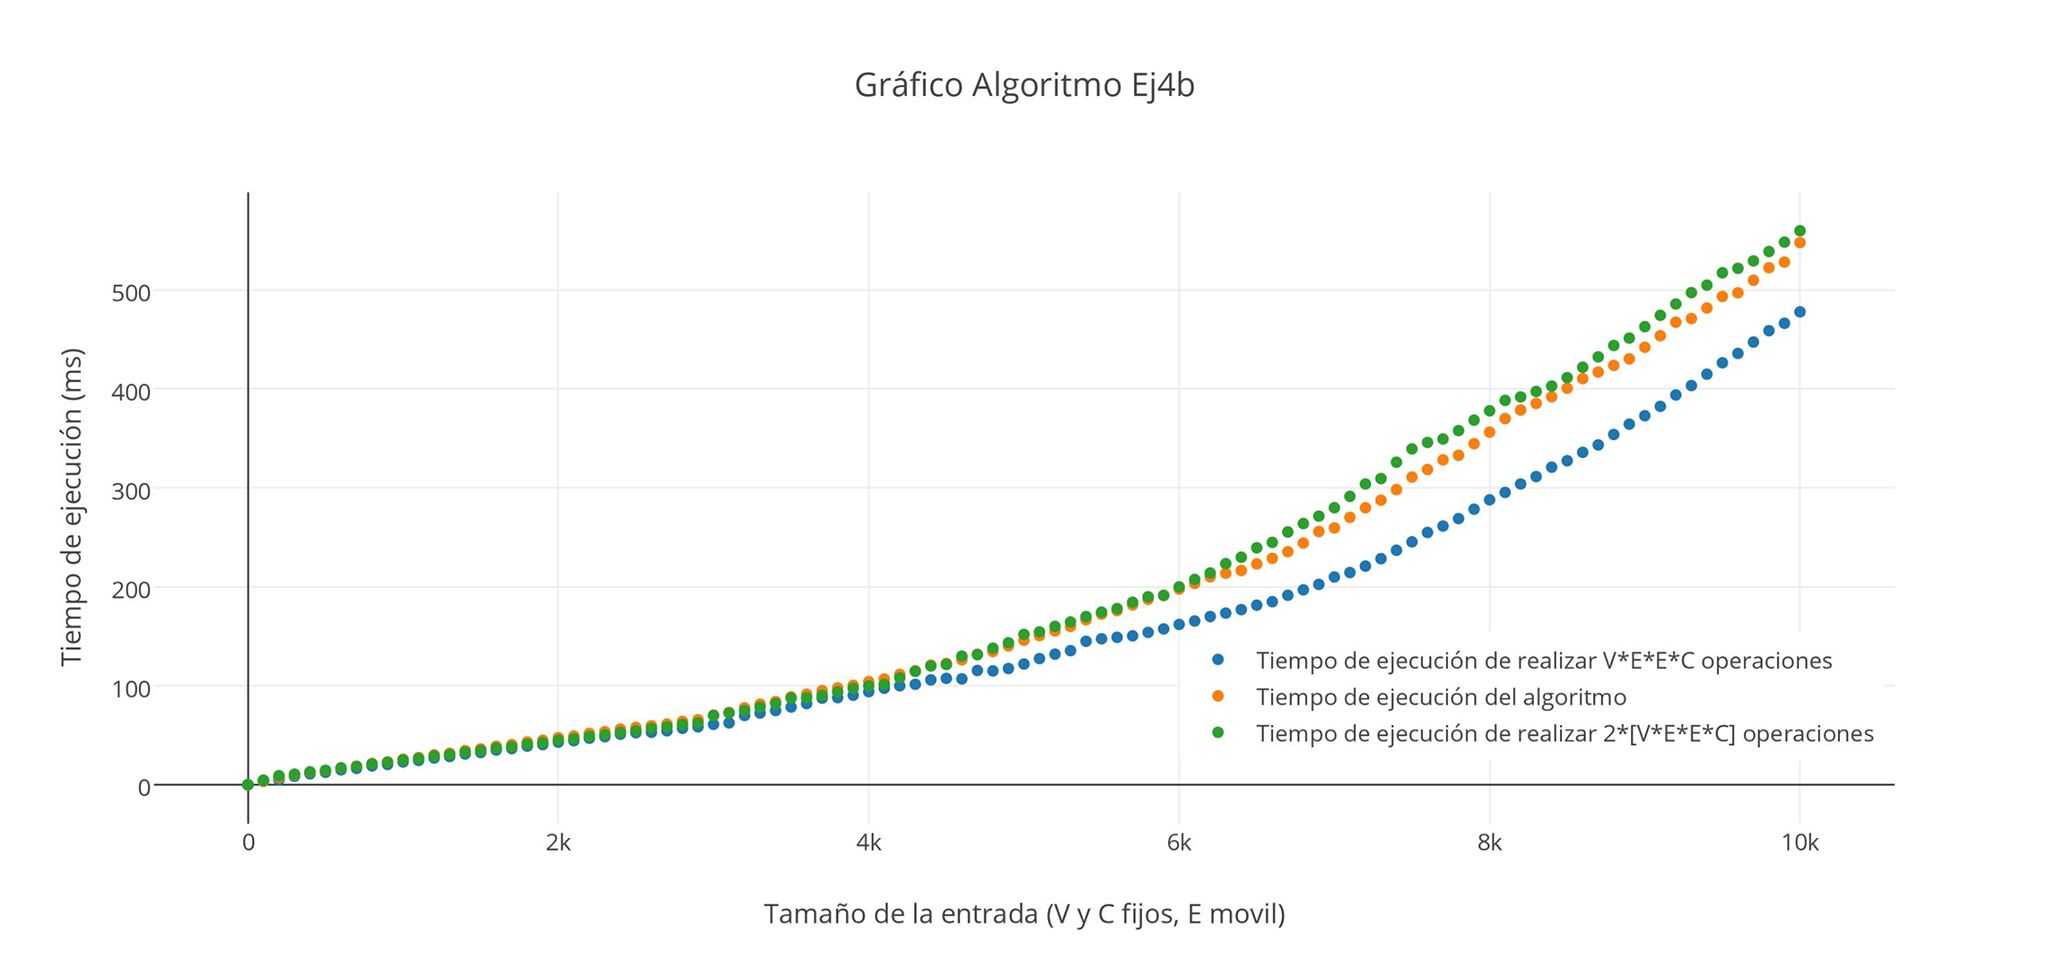
\includegraphics[scale=0.28]{./ej4/completo2b.jpg}
 	{Gráfico 4.4.7 - Medición con grafo completo}
  \end{center}
  \vspace*{0.3cm}

En la figura 4.4.6 se puede observar el tipo de grafo que utilizamos. En la figura 4.4.7, se puede ver como el tiempo de ejecución de nuestro algoritmo es un poco mayor que un grafo circular, ya que tenemos más nodos interconectados y a pesar de esta situación nos mantenemos dentro de los tiempos estipulados corroborando la complejidad calculada.\\

Por último, mostraremos los gráficos comparativos tanto en lo que respecta a porcentajes de soluciones como de tiempos de ejecución:\\
  
  \vspace*{0.3cm} \vspace*{0.3cm}
  \begin{center}
 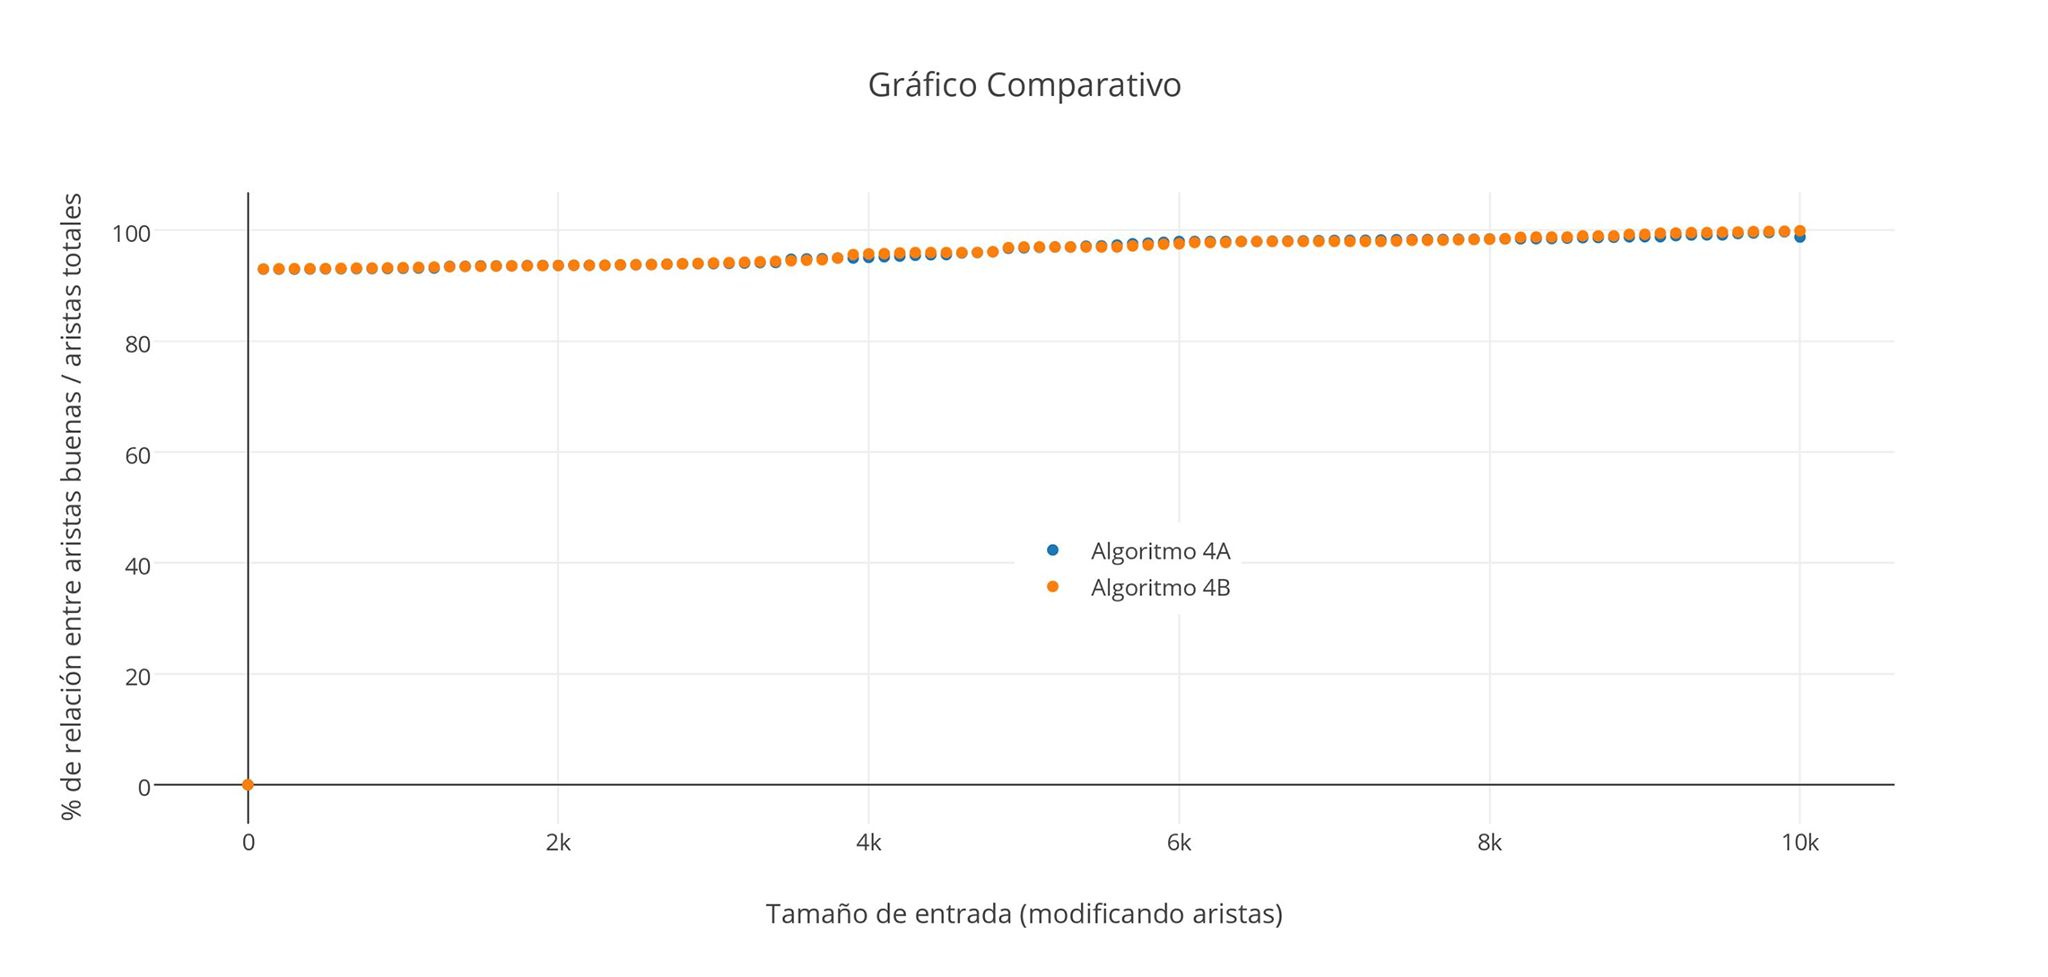
\includegraphics[scale=0.28]{./ej4/comcompleto.jpg}
 	{Gráfico 4.4.9 - Gráfico comparativo algoritmos con grafo completo}
  \end{center}
  \vspace*{0.3cm}
  
En la figura 4.4.9 se observan nuevamente ambas funciones, las cuales simbolizan el porcentaje de realizar la relación entre la cantidad de aristas denominadas buenas sobre la totalidad en un grafo completo. Se puede observar como el algoritmo del inciso b es sensiblemente superior y al incrementarse la cantidad de aristas como el porcentaje de relación aumenta gradualmente dando un alto grado de aristas "buenas" ya que existe menor cantidad de restricciones.\\

Y por último, el gráfico comparativo en función del tiempo de ejecución de los algoritmos para dicho grafo completo.

  \vspace*{0.3cm} \vspace*{0.3cm}
  \begin{center}
 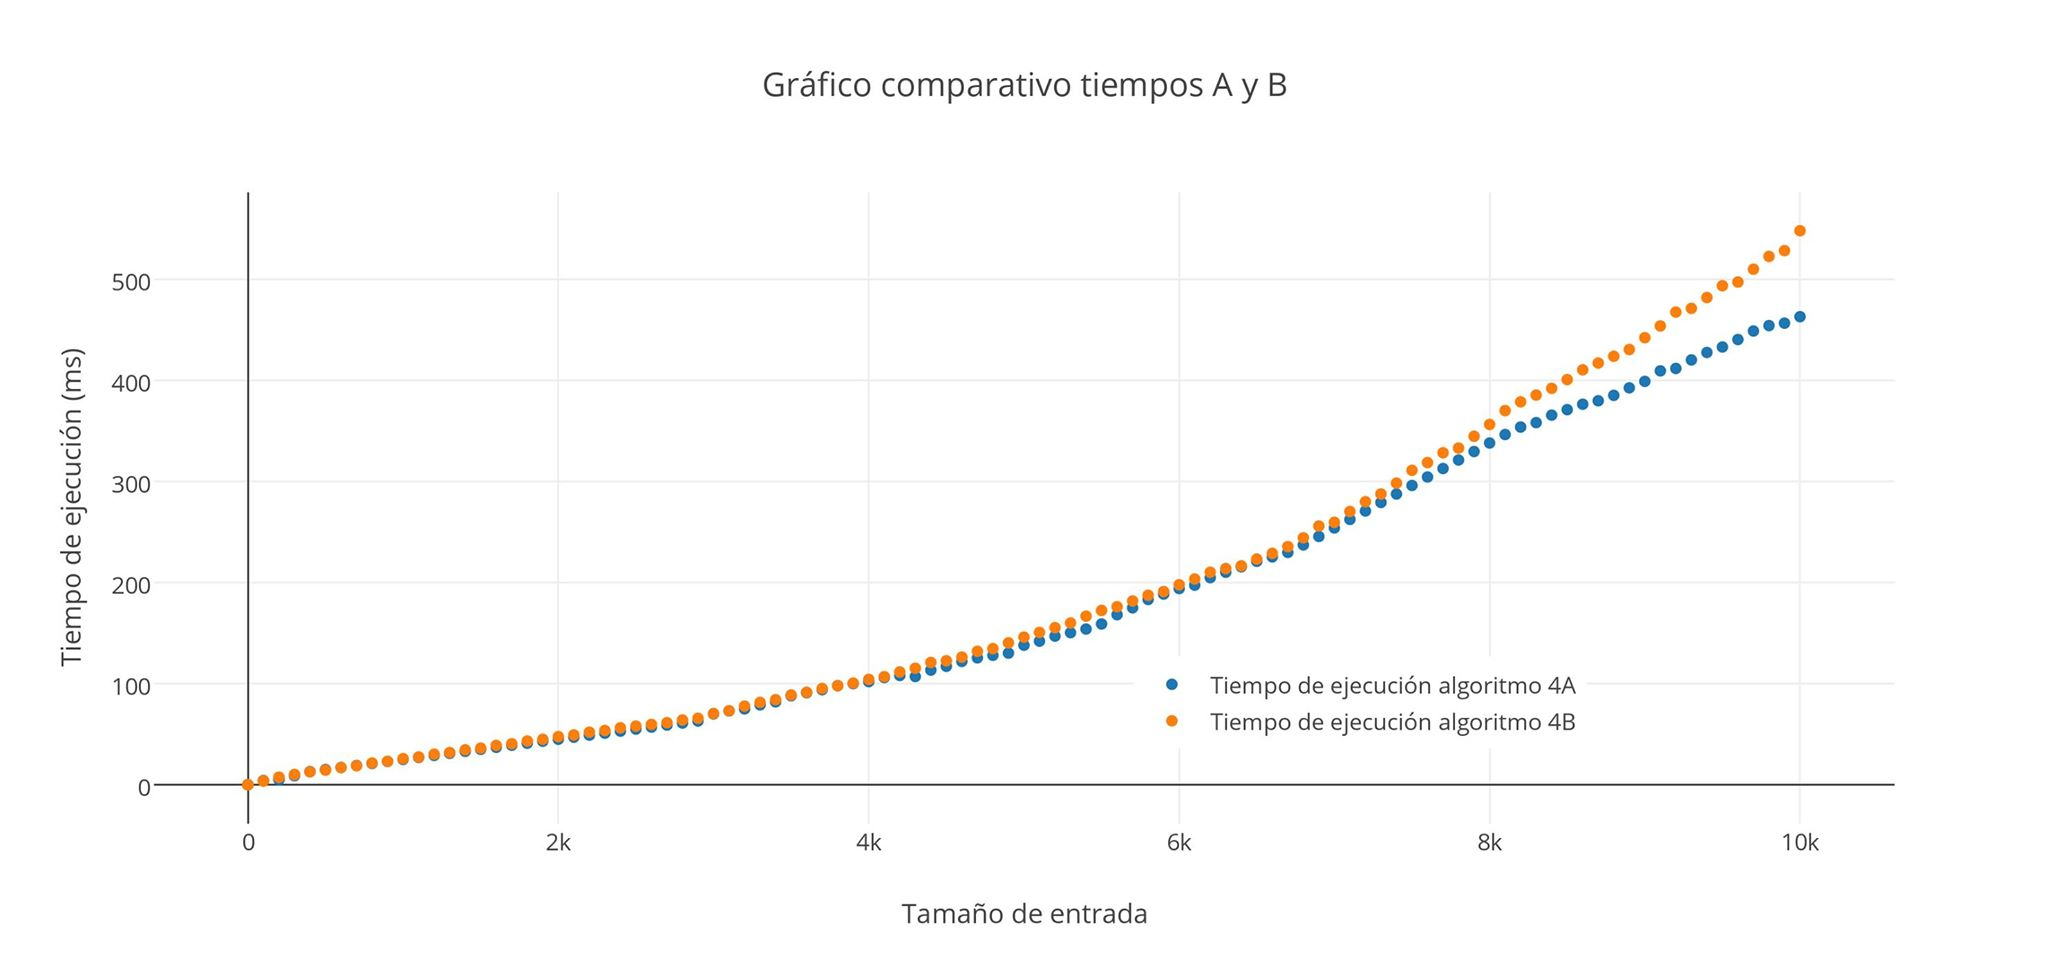
\includegraphics[scale=0.28]{./ej4/comcompleto2.jpg}
 	{Gráfico 4.4.10 - Gráfico comparativo algoritmos con grafo completo}
  \end{center}
  \vspace*{0.3cm}
  
 Se puede observar en las figuras 4.4.10 el tiempo de ejecución de cada algoritmo y como el B insume un poco más de tiempo que el A.\\
 
\subsection{Conclusión comparación entre Vecindades}
Podemos notar que ambas vecindades presentan calidades de solucion similares, mientras que la primera presenta mejor performance de tiempo. Por lo tanto, elegimos esta como vecindad definitiva.